\documentclass{article}
\usepackage[utf8]{inputenc}
\usepackage{subfig}
\usepackage{amsmath}

\usepackage{graphicx}
\usepackage[legalpaper, landscape, margin=0.5cm]{geometry}

\thispagestyle{empty}
% \renewcommand{\thesubfigure}{\roman{subfigure}}
\begin{document}

\begin{figure}[h]
        \centering
        \subfloat[lens sagittal cut]{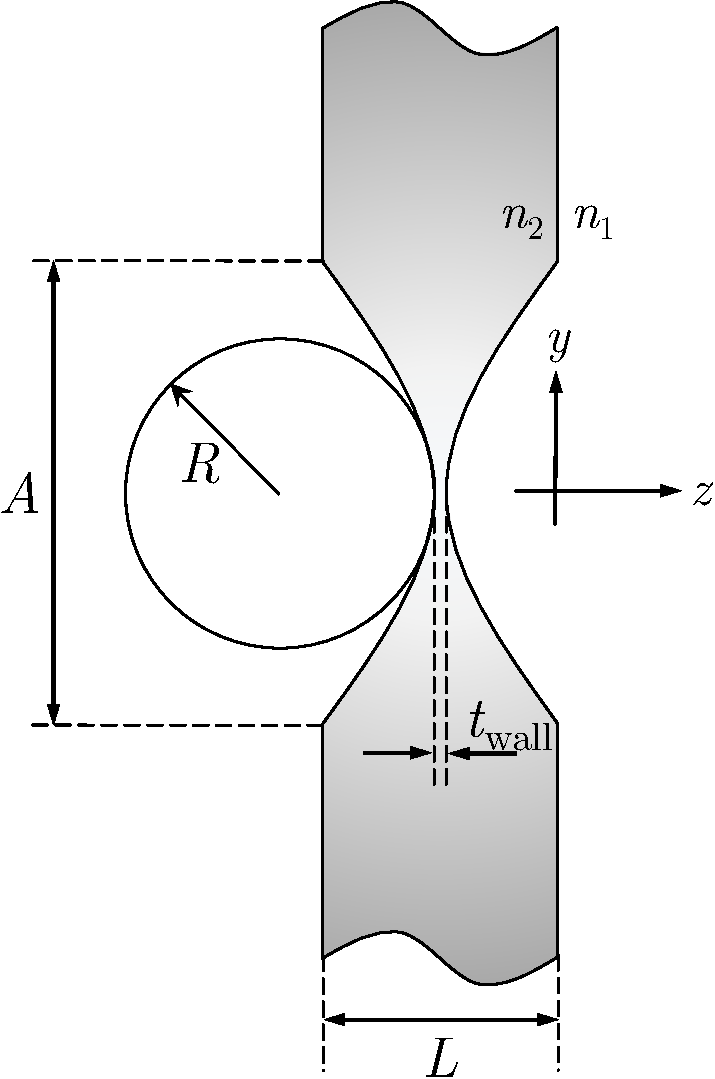
\includegraphics[height=4.6cm]{illu/figures/ch03/lens_01.pdf}}\hspace{0.85cm}
        \subfloat[effect of stacking lenslets]{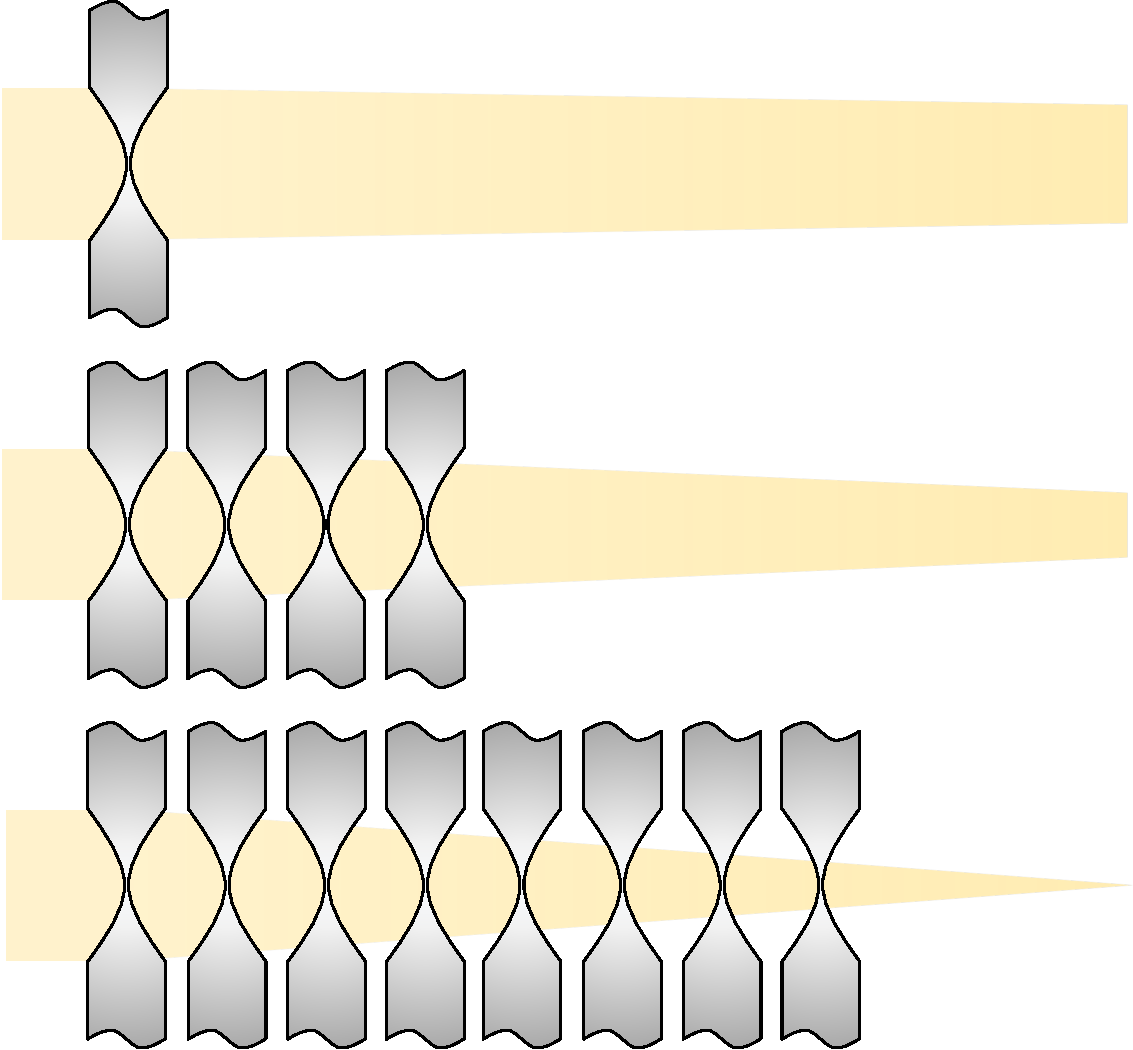
\includegraphics[height=4.6cm]{illu/figures/ch03/lens_02.pdf}}\\
        \subfloat[N-stacked lenses to form a CRL]{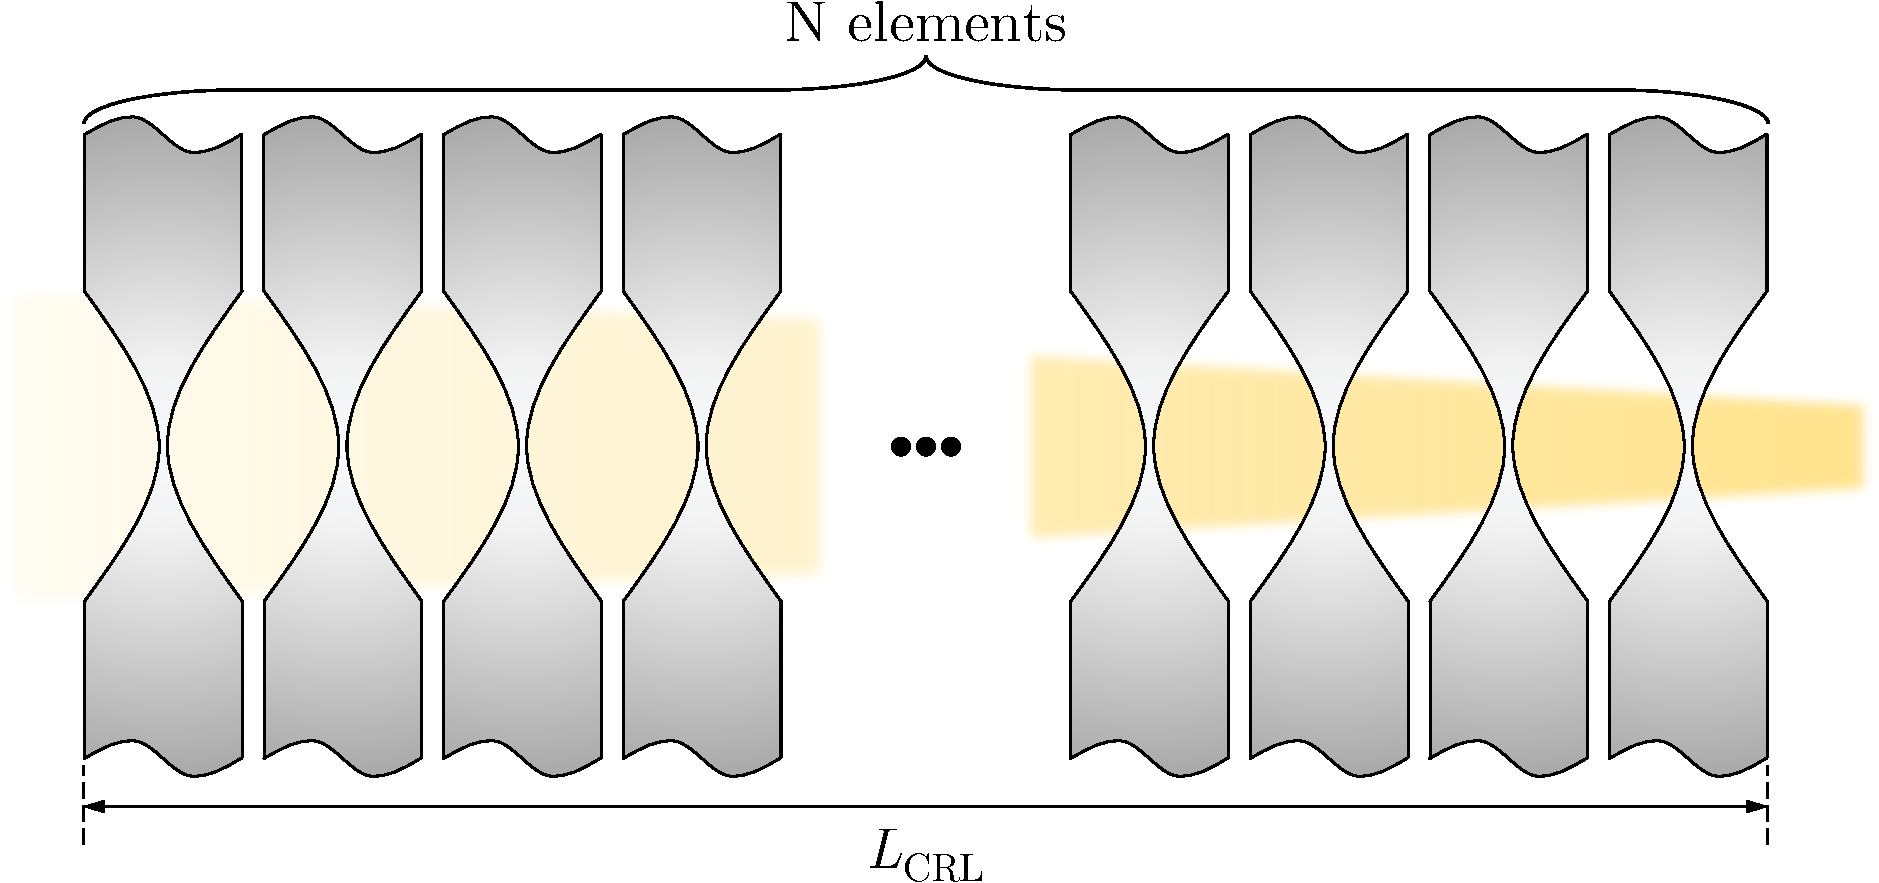
\includegraphics[height=4.0cm]{illu/figures/ch03/lens_03.pdf}}
\end{figure}
\end{document}